\documentclass[a4paper,12pt]{article}

\usepackage{url}
\usepackage{epsfig}
\usepackage{graphics}
\usepackage{fancyhdr}
% \usepackage[backend=bibtex]{biblatex}

\graphicspath{{pictures/}}

\title{Word prediction performance of n-gram models applied to essentially different corpora}
\author{\hspace*{-0.5cm}
GROUP 34\\
\begin{tabular}{cccc}
Sofia Broom\'e & Jeremy Krebs & Valentin Geffrier & Erik Fredriksen \\
901210 & BIRTHDATE2 & BIRTHDATE3 & BIRTHDATE4 \\
sbroome@kth.se & MAIL2@kth.se & MAIL3@kth.se & MAIL4@kth.se \\
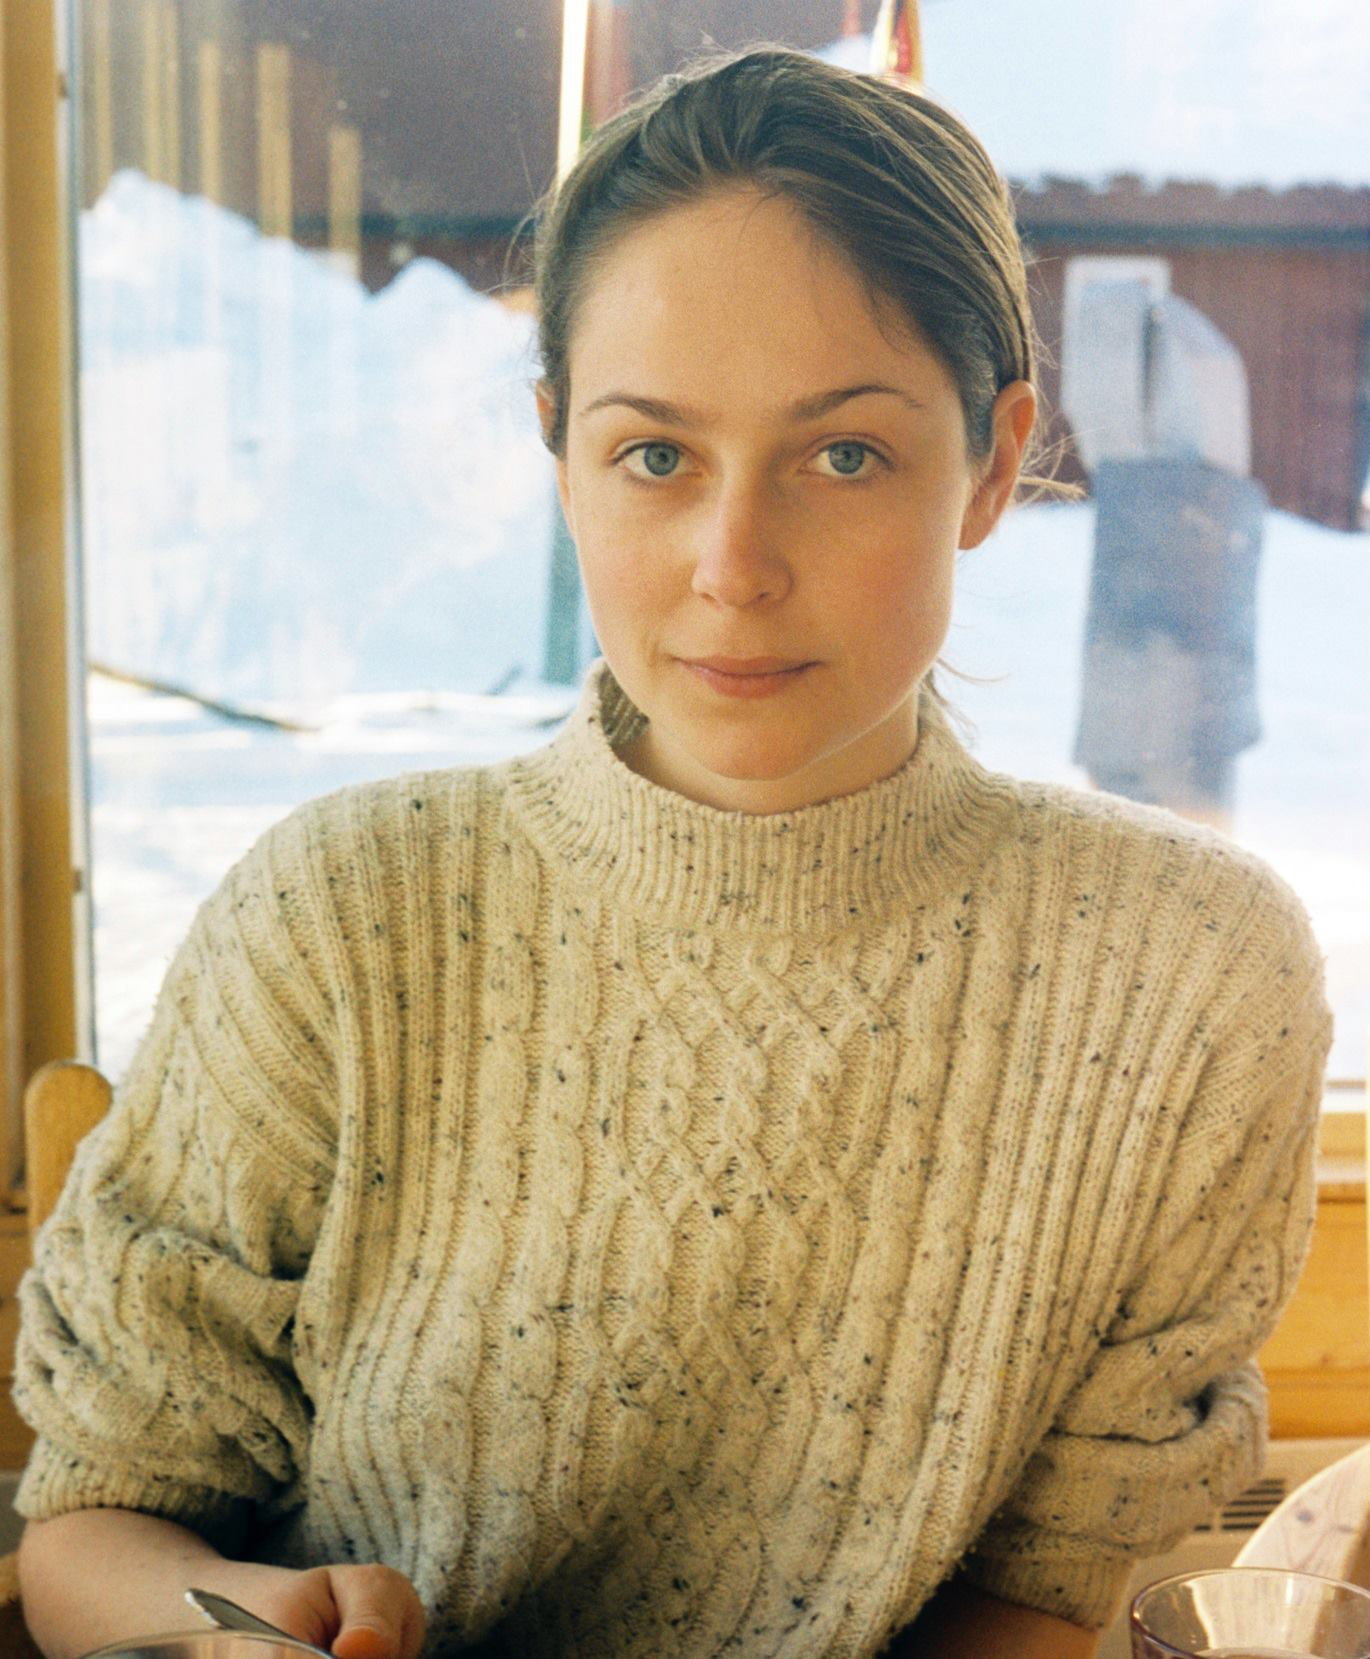
\includegraphics[width=0.13\linewidth]{Nikkaluokta} & 
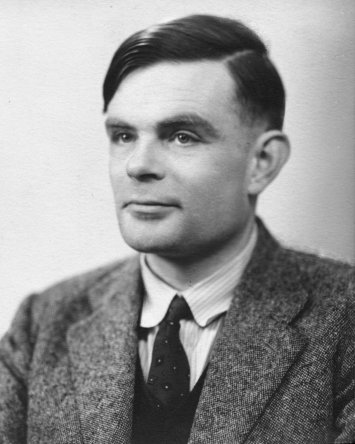
\includegraphics[width=0.13\linewidth]{Alan_Turing_photo} & 
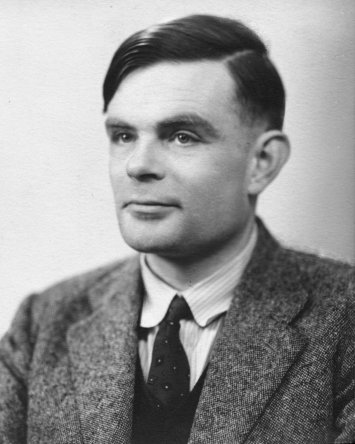
\includegraphics[width=0.13\linewidth]{Alan_Turing_photo} & 
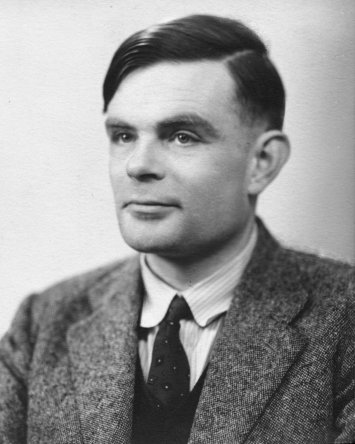
\includegraphics[width=0.13\linewidth]{Alan_Turing_photo}
\end{tabular}} 
% Normally there will not be any pictures but we want
% these so that we can connect faces to names in the course
% We also want birthdates so that we can tell people with the same
% name apart
\date{}

\pagestyle{fancy}
\setlength{\headheight}{15pt}
\fancyhf{}
\lhead{DD2380 ai15} % DO NOT REMOVE!!!!
\rhead{S. Broom\'e, J. Krebs, V. Geffrier, E. Fredriksen} %% UPDATE WITH YOUR NAMES

\begin{document}

\maketitle
\thispagestyle{fancy}

\begin{abstract}
Bla hej bla bla bla bla bla bla bla bla bla bla bla bla bla bla bla bla 
bla bla bla bla bla bla bla bla bla bla bla bla bla bla bla bla bla 
bla bla bla bla bla bla bla bla bla bla bla bla bla bla bla bla bla 
bla bla bla bla bla bla bla bla bla bla bla bla bla bla bla bla bla
\end{abstract}



\clearpage

%%%%%%%%%%%%%%%%%%%%%%%%%%%%%%%%%%%%%%%%%%%%%%%%%%%%%%%%%%%%%
%%%%%%%%%%%%%%%%%%%%%%%%%%%%%%%%%%%%%%%%%%%%%%%%%%%%%%%%%%%%%
\section*{NOTE}
\begin{itemize}

\item The following sections are arranged in the order they would appear in a scientific paper. We think that these sections need to be there and written. However, these are only guidelines and if you think that some of these sections or subsections are irrelevant to you, please feel free to remove them. Similarly, if you want to include more sections or subsections please go ahead. Also feel free to rearrange them according to your convenience, but keeping some common sense (eg.~Introduction cannot come after Conclusions).

\item \textit{Introduction, Related Works, Experimental Results, Discussions, Summary} are sections that MUST be contained.

\item In the section of your \textit{Method}: please do not list your project as log book entries, please talk about the final method you want to present to us. Talk about the method scientifically or technically and not as "I did this..." "Then I tried this..." "this happened...." etc.

\item Do not paste any code unless it is very relevant!

\item The section \textit{Contributions} is a place to express any difference in contributions. The default assumption is that you all agree that all of you had an equal part to play in the project.

\item We suggest that you try to write this as scientifically as possible and not simply like a project report. Good Luck!

\item Please remove \textbf{this} NOTE section in your final report.

\end{itemize}
\section{Introduction (1--2 pages)}
\label{sec:intro}

Being able to dissect, classify, analyze and reproduce language is a highly relevant task for various fields. In the realm of artificial intelligence, we want to give language to our agents by means of communicating with them. When we deal with natural language processing we say that we make language models. Seen as there is no finite set of rules that can describe, say, the entire English language in a complete sense, for pragmatic reasons our best option seems to be basing our models on probabilistic observations - regardless of Noam Chomsky's contempt\cite{JurafskyBook} for the notion of probability of a sentence.

At the foundation of every language model that wants to predict words is the concept of n-grams, a method based on probabilistic distributions over length n combinations of subsequent words. An n-gram is a Markov chain of degree n-1. This quite simple construct can capture many patterns in sentences. Even though it doesn't consider grammar explicitly, grammar will inevitably be built in. For instance, an adjective will in many cases be followed by a noun, or a pronoun by a verb, and thus a bigram composed of those two grammatical types in the mentioned order will score high in probability. 

An n-gram gives us context for words, albeit not the full one. Gao and Suzuki\cite{gao2004long} explore long distance dependency for words through word clusters and the linguistically motivated {\it function word skipping} method where function words such as "has", "a", "in", "and", "the", etc, are skipped in favor of more significant words, called head words. In our experiments however, we will not delve further into this subject.

N-grams can also be used in a meta-sense - for instance it's common for part-of-speech-taggers to use n-gram models where they tag the current word based on the last word's tag.

There are some practical issues with the classical n-gram model. What do we do with the n-grams that aren't in our training set and thus have zero probability assigned? This is where techniques of so called smoothing comes in so that our model doesn't fail on encountering a previously unseen word in the test set. In case we are dealing with a higher-order n-gram and we find it has no probability mass , we might want to "back off" from the higher order and estimate the probability for a conditioned unigram, meaning we temporarily look at a smaller portion of a word's history.

Furthermore, what kinds of test sets does our training set allow us to perform well on? One should train on a  corpus which is representative of the domain of the intended use. And what happens to our model when we apply it to languages with a higher degree of inflection like Swedish, Basque or German?

From the above examples we see that in many cases just using the n-gram model in itself will not suffice. Over the years researchers in natural language processing have added a lot of tweaks to the original idea such as linear combinations of n-gams, cache language models, LSA-based language models and maximum entropy models, to name a few.

In what follows we will explore n-gram models of varying degrees on dito corpora and grammar to see which results are obtained under which circumstances.

\subsection{Contribution}
Bla bla bla bla bla bla bla bla bla bla bla bla bla bla bla bla bla 
bla bla bla bla bla bla bla bla bla bla bla bla bla bla bla bla bla 
bla bla bla bla bla bla bla bla bla bla bla bla bla bla bla bla bla 
bla bla bla bla bla bla bla bla bla bla bla bla bla bla bla bla bla

\subsection{Outline}
Bla bla bla bla bla bla bla Section~\ref{sec:relwork} bla bla bla bla 
bla bla bla bla bla Section~\ref{sec:method} bla bla bla bla bla bla 
bla bla bla bla bla bla bla bla bla bla bla Section~\ref{sec:exps}
bla bla bla bla bla bla Section~\ref{sec:summary} bla bla bla bla bla

%%%%%%%%%%%%%%%%%%%%%%%%%%%%%%%%%%%%%%%%%%%%%%%%%%%%%%%%%%%%%
%%%%%%%%%%%%%%%%%%%%%%%%%%%%%%%%%%%%%%%%%%%%%%%%%%%%%%%%%%%%%
\section{Related work}
\label{sec:relwork}

Bla bla bla bla bla bla bla bla bla bla bla bla bla bla bla bla bla 
bla bla bla bla bla bla bla bla bla bla bla bla bla bla bla bla bla 
bla bla bla bla bla bla bla bla bla bla bla bla bla bla bla bla bla 
bla bla bla bla bla bla bla bla bla bla \cite{RussellNorvigAIBook3rd}
bla bla bla bla bla bla

%%%%%%%%%%%%%%%%%%%%%%%%%%%%%%%%%%%%%%%%%%%%%%%%%%%%%%%%%%%%%
%%%%%%%%%%%%%%%%%%%%%%%%%%%%%%%%%%%%%%%%%%%%%%%%%%%%%%%%%%%%%
\section{My method}
\label{sec:method}

Bla bla bla bla bla bla bla bla bla bla bla bla bla bla bla bla bla 
bla bla bla bla bla bla bla bla bla bla bla bla bla bla bla bla bla 
bla bla bla bla bla bla bla bla bla bla bla bla bla bla bla bla bla 

\subsection{Implementation}
\label{sec:impl}

Bla bla bla bla bla bla bla bla bla bla bla bla bla bla bla bla bla 
bla bla bla bla bla bla bla bla bla bla bla bla bla bla bla bla bla 
bla bla bla bla bla bla bla bla bla bla bla bla bla bla bla bla bla 

%%%%%%%%%%%%%%%%%%%%%%%%%%%%%%%%%%%%%%%%%%%%%%%%%%%%%%%%%%%%%
%%%%%%%%%%%%%%%%%%%%%%%%%%%%%%%%%%%%%%%%%%%%%%%%%%%%%%%%%%%%%
\section{Experimental results}
\label{sec:exps}

Bla bla bla bla bla bla bla bla bla bla bla bla bla bla bla bla bla 
bla bla bla bla bla bla bla bla bla bla bla bla bla bla bla bla bla 
bla bla bla bla bla bla bla bla bla bla bla bla bla bla bla bla bla 

\subsection{Experiemntal setup}
Bla bla bla bla bla bla bla bla bla bla bla bla bla bla bla bla bla 
bla bla bla bla bla bla bla bla bla bla bla bla bla bla bla bla bla 
bla bla bla bla bla bla bla bla bla bla bla bla bla bla bla bla bla 

\subsection{Experiment ...}

Bla bla bla bla bla bla bla bla bla bla bla bla bla bla bla bla bla 
bla bla bla bla bla bla bla bla bla bla bla bla bla bla bla bla bla 
bla bla bla bla bla bla bla bla bla bla bla bla bla bla bla bla bla 

\begin{figure}
\centering
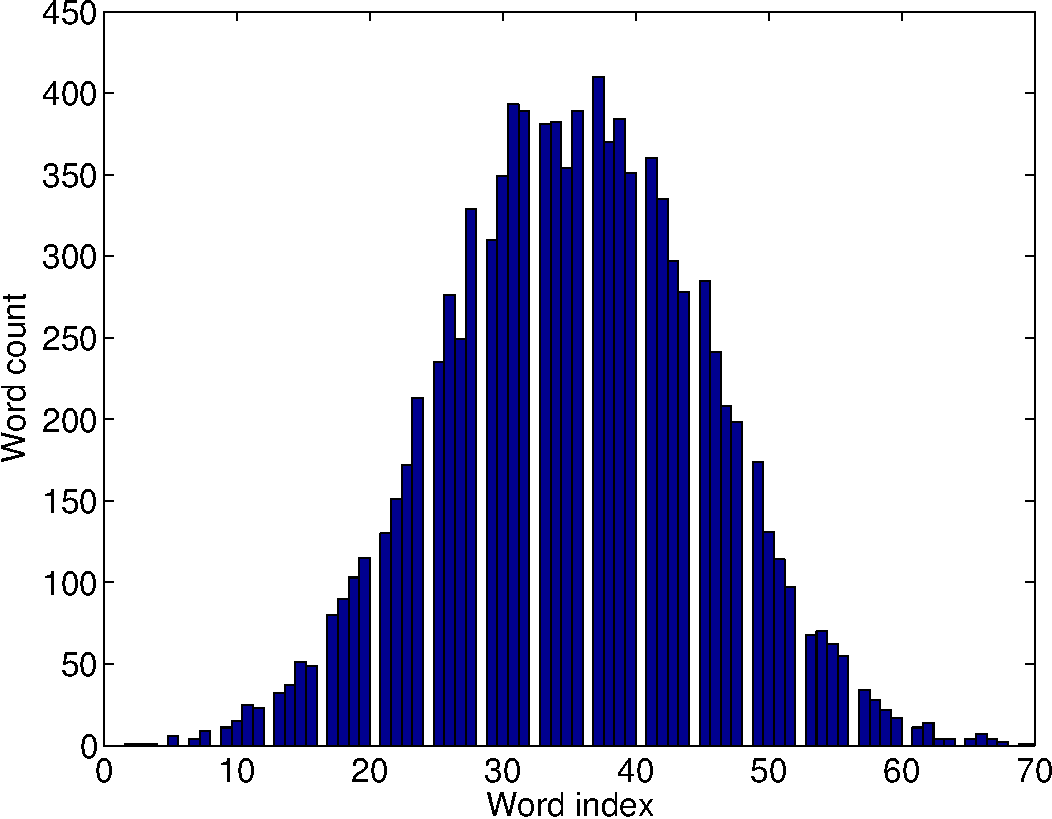
\includegraphics[width=0.8\linewidth]{histogram}
\caption{A description that makes browsing the paper easy and clearly 
describes what is in the picture. Make sure that the text in the figure 
is large enough to read and that the axes are labelled.}
\label{fig:histogram}
\end{figure}

Bla bla bla bla bla Figure~\ref{fig:histogram} bla bla bla bla bla bla 
bla bla bla bla bla bla bla bla bla bla bla bla bla bla bla bla bla 
bla bla bla bla bla bla bla bla bla bla bla bla bla bla bla bla bla 

\begin{table}
\begin{center}
\begin{tabular}{|c|c|c|}
\hline
Bla bla & Bla bla & Bla bla \\ \hline
42 & 42 & 42 \\ \hline
42 & 42 & 42 \\ \hline
\end{tabular}
\caption{A description that makes browsing the paper easy and clearly 
describes what is in the table.}
\label{tab:results}
\end{center}
\end{table}

Bla bla bla bla bla Table~\ref{tab:results} bla bla bla bla bla bla 
bla bla bla bla bla bla bla bla bla bla bla bla bla bla bla bla bla 
bla bla bla bla bla bla bla bla bla bla bla bla bla bla bla bla bla 

%%%%%%%%%%%%%%%%%%%%%%%%%%%%%%%%%%%%%%%%%%%%%%%%%%%%%%%%%%%%%
%%%%%%%%%%%%%%%%%%%%%%%%%%%%%%%%%%%%%%%%%%%%%%%%%%%%%%%%%%%%%
\section{Summary and Conclusions}
\label{sec:summary}

Bla bla bla bla bla bla bla bla bla bla bla bla bla bla bla bla bla 
bla bla bla bla bla bla bla bla bla bla bla bla bla bla bla bla bla 
bla bla bla bla bla bla bla bla bla bla bla bla bla bla bla bla bla 


%%%%%%%%%%%%%%%%%%%%%%%%%%%%%%%%%%%%%%%%%%%%%%%%%%%%%%%%%%%%%
%%%%%%%%%%%%%%%%%%%%%%%%%%%%%%%%%%%%%%%%%%%%%%%%%%%%%%%%%%%%%
\section{Contributions}
\label{sec:contributions}
We the members of project groupXX unanimously declare that 
we have all equally contributed toward the completion of this
project. (PLEASE CHANGE THIS SUITABLY WITH DETAILS, IF IT IS NOT TRUE)


%%%%%%%%%%%%%%%%%%%%%%%%%%%%%%%%%%%%%%%%%%%%%%%%%%%%%%%%%%%%%
%%%%%%%%%%%%%%%%%%%%%%%%%%%%%%%%%%%%%%%%%%%%%%%%%%%%%%%%%%%%%

\nocite{*}
\bibliographystyle{plain}
\bibliography{reflist}



\end{document}